\section{Mininet-Wifi CLI}
Es esta sección se va a recorrer todas las funcionalidades que nos ofrece la CLI ( Command Line Interface) de Mininet-Wifi en la medida que sea posible. A continuación, listamos todos los comandos que están disponibles y documentados en la CLI de Mininet-Wifi.
\begin{itemize}
    \item EOF   %
    \item distance  %
    \item dpctl %
    \item dump %
    \item exit  %
    \item gterm
    \item help
    \item intfs
    \item iperf
    \item iperfudp
    \item links
    \item net  %
    \item nodes
    \item noecho
    \item pingall
    \item pingallfull
    \item pingpair
    \item pingpairfull
    \item ports
    \item px
    \item py
    \item quit   %
    \item sh
    \item source
    \item start
    \item stop
    \item switch
    \item time
    \item x
    \item xterm
\end{itemize}
\subsection{Comando: EOF + quit + exit}
Estos tres comandos se utilizan para lo mismo, salir de la CLI de Mininet-Wifi y terminar la emulación. El código de estos tres comandos no difieren mucho,  son comandos heredados de la CLI de Mininet. EOF y quit terminan haciendo uso de exit al final, por lo que podríamos decir que son un poco repetitivos.
\begin{minted}[]{python}
    def do_exit( self, _line ):
        "Exit"
        assert self  # satisfy pylint and allow override
        return 'exited by user command'

    def do_quit( self, line ):
        "Exit"
        return self.do_exit( line )

    def do_EOF( self, line ):
        "Exit"
        output( '\n' )
        return self.do_exit( line )
\end{minted}
 \subsection{Comando: distance}
 Este comando sirve para medir la distancia entre dos entes de la topología emulada. El uso es muy sencillo, únicamente hay que indicar el nombre dado a cada ente y nos dará la distancia en metros. 
 
 \begin{figure}[!htb]
  \centering
    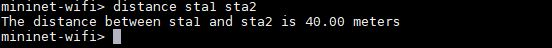
\includegraphics[width=0.8\linewidth]{./img/cli/1.JPG}
    \caption{Comando distance output.}
  \label{fig:yo}
\end{figure}

%% Aquí poner test_topo_1 editada distancia %%

\subsection{Comando: dpctl}
El comando dpctl es un comando heredado de la CLI de Mininet, pero redefinido en el for de Mininet-Wifi con pocas variaciones. Dpctl es un comando de utilidad de administración que permite cierto control sobre el switch OpenFlow (ovs-ofctl en el switch OpenvSwitch). Con este comando es posible agregar flujos a la tabla de flujo, consultar las características y el estado de los switchs y cambiar otras configuraciones, limpiar la tabla entre otras cosas. \newline
\newline
Como se ha dicho este comando tiene bastantes funcionalidades, por no entrar una a una se deja aquí donde se debe ir a consultar cada funcionalidad del comando en función del tipo de switch.
\begin{itemize}
    \item Ofssoftswitch: \url{https://github.com/CPqD/ofsoftswitch13/wiki/Dpctl-Documentation}
    \item OpenvSwitch: \url{http://www.openvswitch.org/support/dist-docs/ovs-ofctl.8.txt}
\end{itemize}
Por lo que se ha podido apreciar en el código del comando, la instrucción se replicará en todos los switches de la topología.
\begin{minted}[]{python}
def do_dpctl(self, line):
        """Run dpctl (or ovs-ofctl) command on all switches.
           Usage: dpctl command [arg1] [arg2] ..."""
        args = line.split()
        if len(args) < 1:
            error('usage: dpctl command [arg1] [arg2] ...\n')
            return
        nodesL2 = self.mn.switches + self.mn.aps
        for sw in nodesL2:
            output('*** ' + sw.name + ' ' + ('-' * 72) + '\n')
            output(sw.dpctl(*args))
            
#Nota: Nosotros utilizaremos sobretodo dpctl dump-flows y 
# dpctl del-flows para consultar o limpiar las tablas de flujo.
\end{minted}

\subsection{Comando: dump + net}
Estos comandos nos arrojarán información sobre la topología emulada. El comando net nos indicará los nombres de los entes que hay en la topología a emular y sus interfaces. El comando dump además nos indicará el tipo de ente, dirección IP, puerto cuando corresponda, interfaz y el identificador de proceso (pid) del ente.

 \begin{figure}[!htb]
  \centering
    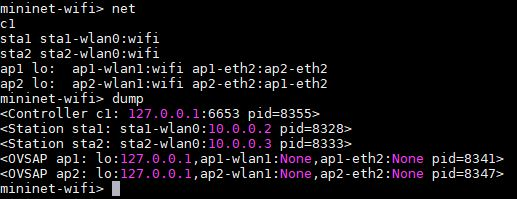
\includegraphics[width=0.8\linewidth]{./img/cli/2.JPG}
    \caption{Comando net y dump output.}
  \label{fig:yo}
\end{figure}
\subsection{Comando: xterm y gterm}

